\chapter{Probabilistic approach}\label{ch:04ProblemFormulation}
\noindent
Given a partial obstacle map, a mission plan, and a small UAV equiped with ADS-B and LiDAR sensor a safe approach to real-time obstacle avoidance with a small computational footprint compatible with the low computational power available in small UAVs. The main application consists of terrain and intruder avoidance for low altitude flights. Following assumption holds:
\begin{enumerate}
  \item There is a obstacle database charting some known obstacles prior the flight.
  \item There is possibility of non-adversarial and non-cooperative intruders.
  \item Estimates of the state of the UAV are available.
  \item The operational space does not contain 'traps' such as caves. 'Traps' arise because the field of view of the LiDAR does not include the whole space surrounding the UAV.
  \item There is a mission plan for the UAV consisting of waypoints which are reachable with vehicle dynamics.
\end{enumerate}
\noindent

\section{Simple plane model}\label{sec:3DsimplisticplaneModel}
\noindent For avoidance theorem formulation in three dimensional space simplified rigid body kinematic model will be used. This model have decoupled roll, yaw and pitch angles which enables to provide simpler and more clean control (e.g movements can be simplified). 

\begin{equation}\label{eq:simple3dStatevector}
    \vec{x} = \left [ x_v,y_v,z_v,\alpha_v,\beta_v,\gamma_v \right ]^T
\end{equation}
State vector (\ref{eq:simple3dStatevector}) defined as positional state in euclidean position in right-hand euclidean space, where $x_v, y_v,z_v$ states, for latitude, longitude and altitude. Orientation angles for vehicle are $\alpha\beta,\gamma$ for roll, pitch, yaw angle.
\begin{equation}\label{eq:simple3dInputVector}
    \vec{u} = \left [ v, \omega_{\alpha_v}, \omega_{\beta_v},\omega_{\gamma_v}\right ]^T
\end{equation}
Input vector (\ref{eq:simple3dInputVector}) is defined as frontal velocity of vehicle $v$,orientation change in main axes as angular speed $\omega_{\alpha_v},\omega_{\beta_v},\omega_{\gamma_v}$
\begin{equation}\label{eq:simple3dvelocityDistribution}
    \begin{bmatrix}
    v_x\\
    v_y\\
    v_z\
    \end{bmatrix}
    = R_{XYZ}(\alpha_v,\beta_v,\gamma_v)
    \begin{bmatrix}
    v\\
    0\\
    0
    \end{bmatrix}
    =
    \begin{bmatrix}
        f_{v_x}(v,\alpha_v,\beta_v,\gamma_v)\\
        f_{v_y}(v,\alpha_v,\beta_v,\gamma_v)\\
        f_{v_z}(v,\alpha_v,\beta_v,\gamma_v)\\
    \end{bmatrix}
    =
    \begin{bmatrix}
         v\cos(\beta_v)\cos(\gamma_v)\\
         v\cos(\beta_v)\sin(\gamma_v)\\
         -v\sin(\beta_v)\\
    \end{bmatrix}
\end{equation}
Velocity distribution function (\ref{eq:simple3dvelocityDistribution}) is is defined trough standard rotation matrix (\ref{eq:xyzspaceRotationMatrix}) and frontal velocity $v$, final distributed velocity is time depending function with values $v_x$, $v_y$, $v_z$ given by functions $f_{v_x}(\dots)$, $f_{v_y}(\dots)$,$f_{v_z}(\dots)$. Final nonlinear model which have been derived from reference model \cite{stevens2015aircraft} is defined by (\ref{eq:simple3ddifferentialequations}).\\
\begin{equation}\label{eq:simple3ddifferentialequations}
    \begin{aligned}
        \dot{x}_v &= v_x  =f_{v_x}(v,\alpha_v,\beta_v,\gamma_v) = v\cos(\beta_v)\cos(\gamma_v)\\
        \dot{y}_v &= v_y  =f_{v_y}(v,\alpha_v,\beta_v,\gamma_v) = v\cos(\beta_v)\sin(\gamma_v)\\
        \dot{z}_v &= v_z  =f_{v_z}(v,\alpha_v,\beta_v,\gamma_v) -v\sin(\beta_v)\\
        \dot{\alpha}_v &= \omega_{\alpha_v}\\
        \dot{\beta}_v &= \omega_{\beta_v}\\
        \dot{\gamma}_v &= \omega_{\gamma_v}\\
    \end{aligned}
\end{equation}

\section{Model predictive control}
\noindent To employ MPC scheme with movement automaton some adjustments needs to be made to original discrete control scheme. These changes are on formal level, because the step time $t_s$ of discrete predictor is similar to fixed movement time $t_i$. So if constraint is satisfied:
\begin{equation}
    t_s = t_{i+1}-t_i, \forall i \in B\in\mathscr{MA} 
\end{equation}
\noindent MPC problem can be solved as discrete time nonlinear MPC problem with fixed discrete time step $t_s = t_{i+1}-t_i$. When movement chain $m_1(t_1),\dots,m_n(t_n)$.
In our case movement automaton $\mathscr{MA}$ is used as input control and state space is constrained by obstacle space $\mathscr{O}$. One can define optimal control problem as follow:
\begin{equation}\label{eq:minProblem}
    \begin{split}
        &\text{Minimize } \sum_{k=0}^{N-1} f_0(k,x(k),u(k)) + \Phi(x(T))\\
        &\text{Subject to: }\\
        &\textit{Dynamics: } x(k+1) = f(k,x(k),u(k)),\quad
        k = 0,1,\dots,T-1\\
        &\textit{Initial conditions: } x(0)= x_0\\
        &\textit{Control constraints: } u(k)\in\mathscr{MA}_i,\quad k = 0,1,\dots
        , T-1\\
        &\textit{State space constraints: } x(k)\in\left\{\mathbb{X}-\mathscr{O}\right\},\quad k = 0,1,\dots
        , T.
    \end{split}
\end{equation}
\noindent Where $\sum_{k=0}^{N-1} f_0(k,x(k),u(k))$ is dynamic control cost functional, $\Phi(x(T))$ is terminal control cost functional. Dynamics of system is given by $f(k,x(k),u(k))$. Initial conditions $x_0$ are considered for initial prediction time $0$ up to finite prediction horizon $H_T$ at time $T$. Control input at time $k$ is considered as time of movement $m(t_i)$ execution time $t_i$. State $x(k)$ is constrained as $x(k)\notin\mathscr{O}$. for any time $k=0,\dots,T$. This problem is modified problem of dynamic programming with constraints.

\subsection{Model predictive control with movement automaton}
\noindent This section describes method used for predictor. The book \cite{durbin2012time} addresses state space modeling of time series. Time series are long term statistical study method. Methods used in time series can be abused to obtain predictor for movement automaton $\mathscr{MA}$. Predictor uses observed state $x$ and known space assessment of avoidance grid $\mathscr{A}(t_i)$ to predict future state chain $\hat{x}$ and movement chain $\hat{B}$. Therefore predictor function is given as follows:
\begin{equation}\label{eq:predictorGlobalForm}
    f:\vec{x}\times \mathscr{A}(t_i)\to \hat{x}\times\hat{B}
\end{equation}
\noindent The main advantage of movement automaton $\mathscr{MA}$ control is separability of input $u$ from state $\hat{x}$. Input signal $u(t)$ is generated as interpretation of movement automaton chain $u(t)=\mathscr{I}(m_1(t_1),\dots,m_i(t_i))$. The system is given by discrete time equation:
\begin{equation}
    x^+= f(x,\mathscr{I}(m_1(t_1),\dots,m_i(t_i)))
\end{equation}
\noindent $\mathscr{I}$ is movement interpretation function. Predictor must therefore satisfy following equation:
\begin{equation}
    \hat{m}_i(t_i) =\mathscr{I}^{-1}(\hat{x}(t_i),\mathscr{I}(m_1(t_1),\dots,m_i(t_{i-1})),\quad \hat{x}(0) = x(t_p)
\end{equation}
\noindent Where $\mathscr{I}^{-1}$ is inverse movement interpretation functor, $\hat{x}(t_i)$ is expected predicted state at time $t_i$ and $m_1(t_1),\dots,m_i(t_{i-1})$ is previously executed movement chain, which can be partially predicted movement chain. Therefore prediction window or receding horizon is variable. The time series are using application of discrete events in state space models, which have been partially linearized. Therefore standard linear model for discrete time $x^+=f(x,u)$ where $u$ is some discrete event set can be abused as movement predictor function  $\mathscr{I}^{-1}$. Implementation example can be found in section \ref{ch:movementAutomatonPredictor}.

\subsection{Predictor corrections}
\noindent For this part assume that system operates in infinite time frame $t\in[t_0,\infty)$. The predictor is giving predicted output $\hat{x}(t)$ and predicted input $\hat{u}(t)$ and is given by following equation for system 
(\ref{eq:simple3ddifferentialequations}):
\begin{equation}
    \hat{\dot{x}}(t_d) f_p(\hat{x}(t_d),\hat{u}(t_d),w(t_d),v(t_d))
\end{equation}
\noindent where $t_d$ is prediction time. Predicted input function $\hat{u}(t_d)$ is disturbed by input disturbance $v(t_d)$ and state disturbance $w(t_d)$. The difference between predicted state and real state increases with time. Main purpose of control is tracking, therefore the tracking deviation should be employed as marginal error function $e_d$.
\begin{equation}
    e_d = \sqrt{\norm{\begin{bmatrix}x_v\\y_v\\z_v\end{bmatrix} -\begin{bmatrix}\hat{x}_v\\\hat{y}_v\\\hat{z}_v\end{bmatrix}}} +\sqrt{\norm{\begin{bmatrix}\beta_v\\\gamma_v\end{bmatrix}-\begin{bmatrix}\hat{\beta}_v\\\hat{\gamma}_v\end{bmatrix}}}
\end{equation}
\noindent This error is accumulating prediction $\hat{x}(t_c)$, $\hat{u}(t_c)$ deviation from real input $u(t_c)$ and state vector at time of comparison $t_c$. The marginal error function $e_m$ is in respective notation of system (\ref{eq:simple3ddifferentialequations}). To compare deviation some well established parameter needs to be used. The ideal candidate is safety margin $s_m$, because some partition of safety margin is prediction error, therefore the hard condition for correction is $\frac{1}(12)s_m$. Time of comparison is possible at any execution time $t$, but the correction is possible only at movement automaton switching time when movements $m_{i-1}(t_{i-1}),m_i(t_i)$ are switching. Let us define time of prediction $t_{p1}$ and time of correction $t_{p2}$ with following constraints $t_{p1}\le t_c \le t_{p2}$. then movement chain at time of original prediction $B(t_{p1})=\{m_1^{p1}(t_{1_{p_1}}),\dots, m_\infty^{p1}(t_{t_{p_1}+\infty})\}$ and new chain for time of new prediction $t_{p2}$ to be chained after time of correction $t_c$ given as $B(t_{p2})=\{m_1^{p2}(t_{1_{p_2}}),\dots, m_\infty^{p2}(t_{t_{p_2}+\infty})\}$. Then the final controller input $B$ is given as following equation:
\begin{equation}
    B_{\mathscr{MA}} = \bigcup_{p=\{p_1(t_1),\dots,p_N(t_n)\}}^{c=\{t_{c_1},\dots,t_{c_{N-1}}\}} \left\{m_{1,p}(t_{1,p}),\dots,m_{c,p}(t_{c,p}),\dots,m_{k_p,p}(t_{k_p,p})\right\}
\end{equation}
\noindent Where $p=\{p_1(t_1),\dots,p_N(t_n)\}$ is chain of predictions $c=\{t_{c_1},\dots,t_{c_{N-1}}\}$ is chain of corrections. The prediction $p_i$ is followed by correction $c_i$ if necessary. Movement chain $m_{1,p}(t_{1,p}),\dots,m_{c,p}(t_{c,p}),\dots,m_{k_p,p}(t_{k_p,p})$ denotes that some movements from previous prediction $p_i$ are executed after correction $c_i$ and then new prediction $p_{i+1}$ is employed. The duration of prediction sequences may differ and its denoted by $k_p$ which marks last executed movement executed from prediction $p$. Movement $m_{c,p}(t_{c,p})$ denotes movement executed from chain $p_i$ at time of correction $c_i$. The goal of predictive control quality is to $\text{lim}_{t\to\infty} k_p = \infty$. This has been achieved in simulation. Unfortunately no disturbances were present to employ this approach. Moving receding horizon is known from literature \cite{rawlings1993stability}, it has been modified for movement automaton $\mathscr{MA}$ as shown in this section.

\section{Movement automaton predictor}\label{ch:movementAutomatonPredictor}
\noindent Vehicle system is given by model from section \ref{sec:3DsimplisticplaneModel}. Vehicle control is defined as movement automation $\mathscr{MA}$.  Movement predictor needs to be developed in order to obtain control signal $u(t)$ It is possible to predict movement buffer $B_{\mathscr{MA}}$, 

Vehicle state $x(t_0)$ at start of mission execution is known. Vehicle state in discrete time $x(t)$ is given by equation \ref{eq:vehicleStateDiscreteKnown}. Where $x_v(t),y_v(t),z_v(t)$ is vehicle position in local coordinate frame and $\alpha_v(t),\beta_v(t),\gamma_v(t)$ is vehicle orientation angles.
\begin{equation}\label{eq:vehicleStateDiscreteKnown}
    x(t) = [x_v(t),y_v(t),z_v(t),\alpha_v(t),\beta_v(t),\gamma_v(t)]^T;
\end{equation}
Base movement table for movements $m_i(1)\in M$ have been measured on system model (\ref{sec:3DsimplisticplaneModel}). This table represents vehicle position and orientation differences after execution of movement. Vehicle initial state was set at center of local coordinate frame with narrow orientation $[x_0,y_0,z_0]=[0,0,0]$. Vehicle initial orientation was aligned with main frame axis X, therefore initial orientation angles are $[\alpha_0,\beta_0,\gamma_0] = [0,0,0]$. Vehicle velocity was set to constant value $v_v = 1 ms^{-1}$. Vehicle position after movement execution is given by parameters $x_b,y_b,z_b$ at time $t+1$. Vehicle orientation is given by parameters $\alpha_b,\beta_b,\gamma_b$. Givem parameters are also absolute shifting, because initial state is $[x_0,y_0,z_0,\alpha_b,\beta_b,\gamma_b]$ set to $\vec{0}$.
\begin{table}[H]
    \centering
    \begin{tabular}{|l||c|c|c|c|c|}
    \hline
        $v_x/m_i$           &    Straight  & Down & Up & Left  & Right   \\\hline\hline
        $x_b [m]$           &    1.00	  & 0.98  & 0.98  & 0.98 & 0.98  \\\hline
        $y_b [m]$           &    0	      & 0	  & 0	  & 0.13 & -0.13 \\\hline
        $z_b [m]$           &    0	      & -0.13 & 0.13  &	0	 & 0     \\\hline
        $\alpha_b [rad]$	&    0	      & 0	  & 0	  & 0    & 0     \\\hline
        $\beta_b [rad]$     &    0	      & 0.2   & -0.26 & 0	 & 0     \\\hline
        $\gamma_b [rad]$    &    0	      & 0	  & 0	  & 0.26 & -0.26 \\\hline
    \end{tabular}
    \caption{Base values for movement application, vehicle position difference $x_v,y_v,z_v$ and orientation differences $\alpha_v,\beta_v,\gamma_v$.}
    \label{tab:movementPredictor}
\end{table}
\begin{table}[H]
    \centering
    \begin{tabular}{|l||c|c|c|c|}
    \hline
        $v_x/m_i$           & Down-Left & Down-Right & Up-Left  & Up-Right   \\\hline\hline
        $x_b [m]$           & 0.76  & 0.76  & 0.76 & 0.76  \\\hline
        $y_b [m]$           & -0.13	& 0.13	& 0.13 & -0.13 \\\hline
        $z_b [m]$           & -0.13 & -0.13 & 0.13 & 0.13  \\\hline
        $\alpha_b [rad]$	& 0	    & 0	    & 0    & 0     \\\hline
        $\beta_b [rad]$     & -0.26 & -0.26 & 0.26 & 0.26     \\\hline
        $\gamma_b [rad]$    & 0.26	& -0.26	& 0.26 & -0.26 \\\hline
    \end{tabular}
    \caption{Base values for movement application, vehicle position difference $x_v,y_v,z_v$ and orientation differences $\alpha_v,\beta_v,\gamma_v$.}
    \label{tab:movementPredictor2}
\end{table}
\noindent With defined base movement tables (tab. \ref{tab:movementPredictor}., \ref{tab:movementPredictor2}.) with defined shifting for movement at time $t_0+1$, \textit{rotation} (\ref{eq:rotationSimplisticPredictor}) and \textit{shifting} (\ref{eq:shiftingSimplisticPredictor}) equations must be defined in order to obtain predicted position $\hat{x}(t+1)$. Position after movement execution $[\hat{x}(t+1),\hat{y}(t+1),\hat{z}(t+1)]$ is depending on vehicle orientation before movement execution $[\alpha_v(t),\beta_v(t),\gamma_v(t)]$. Rotation function rotates vehicle position $[x_b(t_0),y_b(t_0),z_b(t_0)]$ according to vehicle orientation angles $[\alpha_v(t),\beta_v(t),\gamma_v(t)]$. For rotation standard rotation matrix $R_{XYZ}(\alpha,\beta\gamma)$ (\ref{eq:xyzspaceRotationMatrix}) is used. Final position offset vector $[\tilde{x}_b(t+1),\tilde{y}_b(t+1),\tilde{z}_b(t+1)]$ at predicted time $t+1$ is given by equation \ref{eq:rotationSimplisticPredictor}.
\begin{equation}\label{eq:rotationSimplisticPredictor}
    \begin{bmatrix}
        \tilde{x}_b\\ 
        \tilde{y}_b\\
        \tilde{z}_b\\
    \end{bmatrix}
    = R_{XYZ}(\alpha_v(t),\beta_v(t),\gamma_v(t))
    \begin{bmatrix}
        x_b\\ 
        y_b\\
        z_b\\
    \end{bmatrix}
\end{equation}
Predicted state vector $\hat{x}(t+1)$ a at time $t+1$ is obtained by combining position offset vector $[\tilde{x}_b(t+1),\tilde{y}_b(t+1),\tilde{z}_b(t+1)]$, orientation offset vector $\alpha_b(t+1),\beta_b(t+1),\gamma_b(t+1)$. as given in equation \ref{eq:shiftingSimplisticPredictor}.
\begin{equation}\label{eq:shiftingSimplisticPredictor}
    \begin{aligned}
    \hat{x}(t+1) & = [\hat{x}_v(t+1),\hat{y}_v(t+1),\hat{z}_v(t+1),\hat{\alpha}_v(t+1),\hat{\beta}_v(t),\hat{\gamma}_v(t)]^T\\
    \hat{x}_v(t+1) & = x_v(t)+\tilde{x}_b\\
    \hat{y}_v(t+1) & = y_v(t)+\tilde{y}_b\\
    \hat{z}_v(t+1) & = z_v(t)+\tilde{z}_b\\
    \hat{\alpha}_v(t+1) & = \alpha_v(t) + \alpha_b\\
    \hat{\beta}_v(t+1) & = \beta_v(t) + \beta_b\\
    \hat{\gamma}_v(t+1) & = \gamma_v(t) + \gamma_b
    \end{aligned}
\end{equation}
Movement automaton $\mathscr{MA}$ has chaining property, therefore movement prediction chaining is also possible via recursive procedure for discrete execution time $t_i$. There exist predicted movement buffer $\hat{B}$ with ordered movement sequence $m_1(1),\dots,m_i(1)$, vehicle state after applying movement $m_{i+1}$ at time $t_i$ can be obtained via equation \ref{eq:discretePredictionChaining}.
\begin{equation}\label{eq:discretePredictionChaining}
    \hat{x}(t_i+1) = f(\hat{x}(t_i),m_{i+1}(1))
\end{equation}
Prediction function $f(\hat{x}(t_i),m_{i+1}(1))$ is in this case function defined by equation \ref{eq:shiftingSimplisticPredictor}, where parameters $[x_b,y_b,z_b,\alpha_b,\beta_b\gamma_b]$ are selected based on movement $m_{i+1}(1)$ type from look-up tables  \ref{tab:movementPredictor}., \ref{tab:movementPredictor2}.



\section{General algorithm}\label{sec:general algorithm}
\noindent General algorithm describes how final probabilities for cell and trajectory are calculated. It shows how time continuum impacts various partial ratings. This section is situated at one specific time of avoidance $t_i$. 

\emph{Obstacle probability} $P_O\in[0,1]$ for cell $c_{i,j,k}$ have been identified during analysis. Later on partial probabilities of \emph{map obstacle} $P_{O_M}$, \emph{detected obstacle} $P_{O_D}$, and \emph{aggregated intruders probability} $P_{O_I}$ will be introduced. The final obstacle probability $P_O$ for one cell $c_{i,j,k}$ is given as:
\begin{equation}
    P_O = 1- \left \{ (1-P_{O_I})\times (1-P_{O_M}) \times (1-P_{O_D})\right \}
\end{equation}
\noindent The obstacle probability $P_O$ for cell $c_{i,j,k}$ is given as inverted product of \emph{intruder obstacle probability} $P_{O_I}$ (sec. \ref{sec:intruderIntersectionModel}), \emph{detected obstacle probability} $P_{O_D}$ (sec. \ref{sec:detectedObstacleProbability}), and \emph{Map obstacle probability} $P_{O_M}$ (sec. \ref{sec:mapObstacleProbability}).


\emph{Visibility probability} $P_V$ for cell $c_{i,j,k}$ is defined in section \ref{sec:visibilityProbability}. The calculation principle is to count LiDAR beams passed trough cell $c_{i,j,k}$ to count of possibly passing $LiDAR$ beams. The meaning of this rating is to show how good was visibility of space portion contained by cell $c_{i,j,k}$.

\emph{General algorithm} inputs and initialization is given by eq. \ref{eq:mainRatingInputs}. The set of intruders $\mathscr{I}$ is set of detected intruders in time frame $[t_{i-1},t_i)$, where $t_{i-1}$ is previous passed avoidance (decision) time and $t_i$ upcoming decision time. The initial position of intruders is projected to upcoming decision time $t_i$. 

\emph{Map obstacle set} $\mathscr{O}_m$ is loaded from obstacle database via \emph{radius select} to expected vehicle position $\hat{x}(t_i)\to\mathscr{F}_{3D}$.

\emph{Detected obstacle set} $\mathscr{O}_d$ is gathered from vehicle sensor systems in time interval $[t_{i-1},t_i)$. The obstacles are steam-lined to avoidance grid $\mathscr{A}(t_i)$ at expected vehicle position $\hat{x}(t_i)\to\mathscr{F}_{3D}$.

\emph{Reach set} $\mathscr{R}$ (set of trajectories) is integral part of avoidance grid $\mathscr{A}(t_i)$ and contains trajectories bounded by $\mathscr{A}(t_i)$ from expected vehicle position $\hat{x}(t_i)\to\mathscr{F}_{3D}$ Each trajectory has ordered set of passing cells $\mathscr{C}(\mathscr{T}(\vec{x},B))$.

\emph{Avoidance grid} $\mathscr{A}(t_i)$ is partitioned into cells $c_{i,j,k}$, $i\in{1..a}$, $j\in{1..b}$, $k\in{1..c}$, $a,b,c\in\N^+$. There exist homogeneous partition of field of vision and cell space is given by:
\begin{equation}
    c_{i,j,k}\to\R^3=\left\{\vec{p}=[d,\theta,\varphi]\in\R^3:\begin{aligned}d_i \le d\le d_{i+1}\\\theta_i\le\theta\le\theta_{i+1}\\\varphi_i\le\varphi\le\varphi_{i+1}\end{aligned}\right\}
\end{equation}
\noindent The cell space is non-inclusive space in local coordinates with origin at vehicle state $\hat{x}(t_i)\to\R^3$ and with main axis (X) at vehicle heading in right hand coordinate frame. The cell space is same as in deterministic approach. Each cell has \emph{passing trajectory set} $\mathscr{T}(c_{i,j,k})$ containing passing trajectories. 

\emph{Initialization} phase is executed every avoidance time $t_i$, the initialization is executed in following manner:
\begin{enumerate}
    \item \emph{Grid cell} $\forall c_{i,j,k}\in\mathscr{A}(t_i)$ - visibility probability $P_V$ is set to 1, because its assumed that all of avoidance grid $\mathscr{A}(t_i)$ is visible, obstacle probability $P_O$ is set to 0 because its expected that all space contained by avoidance grid $\mathscr{A}(t_i)$ is free.
    \item \emph{Trajectory} $\forall \mathscr{T}(\vec{x},B)\in\mathscr{R}(\vec{x},t_i,t_{i+1})$ - For each trajectory segment $s\subset B$ passing trough cell set $\mathscr{C}(\mathscr{T}(\vec{x},s))$ the \emph{reachability probability} $P_R(\mathscr{T}(\vec{x},s))$ is initialized to 1, due the properties of space contained in $\mathscr{C}$ (visible, free of obstacles).
\end{enumerate}

\begin{equation}\label{eq:mainRatingInputs}
    \begin{aligned}
    \textbf{\textit{Inputs:}}\quad&\textit{Intruders}&\quad\mathscr{I}=\left\{I_1,\dots ,I_A\right\}\\
    &\textit{Map obstacles}&\quad \mathscr{O}_m=\left\{o_{m,1},\dots,o_{m,B}\right\}\\
    &\textit{Detected obstacles}&\quad \mathscr{O}_d=\left\{o_{d,1},\dots,o_{d,C}\right\}\\
    &\textit{Reach set (trajectories)}&\quad \mathscr{R}=\left\{\mathscr{T}_1,\dots,\mathscr{T}_D\right\}\\
    &\textit{Avoidance grid}& \quad \left\{c_{1,1,1},\dots,c_{I,J,K}\right\}\in\mathscr{A}(t_i)\\
    \textbf{\textit{Initialize:}}\quad&\forall c_{i,j,k}\in\mathscr{A}(t_i)&\quad P_O = 0 , \quad P_V = 1\\
    &\forall \mathscr{T}_d\in\mathscr{R}&\quad P_R = 1\\
    \end{aligned}
\end{equation}
\begin{equation}\label{eq:mainRatingCalculation}
    \begin{aligned}
    1.&\text{Propagate intruders } \mathscr{I} \text{, map obstacles } \mathscr{O}_m \text{, detected obstacles }\mathscr{O_d}\text{,}\\
      &\text{trough avoidance grid } \mathscr{A}(t_i) \text{ so each cell } c_{i,j,k} \text{ has obstacle } P_O\\
      &\text{and visibility } P_V \text{ probability set.}\\
    2.&\text{For each trajectory } \mathscr{T}_d\in\mathscr{R} \text{ and for each point of trajectory,}\\
      &\text{calculate reachability probability } P_R \text{ given by (\ref{eq:TrajectoryReachibilityAtPoint}).}\\
    3.&\text{For each cell } c_{i,j,k} \text{ in avoidance grid, there exists set of}\\
      &\text{passing trajectories } \mathscr{T}\in c_{i,j,k}=\left\{\mathscr{T_f}\in\mathscr{R}|(\mathscr{T}_f\to\R^3)\cap c_{i,j,k} \neq 0\right\}\text{.}\\
    4.&\text{Reachibility probability } P_R \text{ calculated for each cell} c_{i,j,k} \\
      &\text{ is given  by(\ref{eq:CellReachibilityGeneral}).}\\
    \end{aligned}
\end{equation}

\noindent\emph{General algorithm} is given by eq. \ref{eq:mainRatingCalculation}. the outputs of algorithm the final reachability probability of trajectories $\mathscr{T}(\vec{x},B)$ in reach set approximation $\mathscr{R}(\vec{x},t_i,t_{i+1})$ is given by definition \ref{def:ReachibilityProbabilityForTrajectory}. When \emph{reachability probability} for all trajectories at all intersection points are assessed, it is possible to assess \emph{reachability probability} $P_R(c_{i,j,k})$ for all cells $c_{i,j,k}$ in avoidance grid $\mathscr{A}(t_i)$. \emph{Cell reachability probability} $P_R(c_{i,j,k})$ in avoidance grid $\mathscr{A}(t_i)$ is given by definition \ref{def:cellReachibilityProbability}.

\begin{definition}{Reachibility probability of trajectory}\label{def:ReachibilityProbabilityForTrajectory} $\mathscr{T}(\vec{x},B)$ in reach set approximation $\mathscr{R}(\vec{x},t_i,t_{i+1})$ in avoidance grid $\mathscr{A}(t_i)$ at time of avoidance $t_i$. There exists ordered set of passing cells $\mathscr{C}$ (\ref{eq:passingCellSequence}).  
    \begin{equation}\label{eq:passingCellSequence}
        {c_{i_1,j_1,k_1},c_{i_2,j_1,k_1},\dots,c_{i_n,j_n,k_n}}=\mathscr{C}\subset\mathscr{A}(t_i)
    \end{equation}
Passing cells set $\mathscr{C}$ is ordered and hierarchical $i_1\le i_2 \le \dots \le i_n$, $i_1,\dots,i_n\in\N^+,n>1$. Each cell $c_{i,j,k}\in\mathscr{C}$ has assessed obstacle $P_O(c_{i,j,k})$ and visibility probability $P_V(c_{i,j,k})$. Then for trajectory $\mathscr{T}(\vec{x},B)$ is probability of reachability $P_R\left ( \mathscr{T}\right)$ given as (\ref{eq:TrajectoryReachibilityAtPoint}).
    \begin{equation}\label{eq:TrajectoryReachibilityAtPoint}
        P_R\left ( \mathscr{T}\right )=\prod_{c_{i,j,k}\in\mathscr{C}(\mathscr{T})}\left(1-P_O(c_{i,j,k}).P_V(c_{i,j,k})\right)
    \end{equation}
\end{definition}


\begin{definition}{Cell reachability probability}\label{def:cellReachibilityProbability} $P_R(c_{i,j,k})$ in avoidance grid $\mathscr{A}(t_i)$ at time of avoidance $t_i$ have set of passing trajectories $\mathscr{T}\in c_{i,j,k}$ with assessed trajectory reachability probability $P_R(\mathscr{T}(\vec{x},B))$ (def. \ref{def:ReachibilityProbabilityForTrajectory}). Then the final cell reachability probability $P_R(c_{i,j,k})$, which is base in cell goal determination, is given as maximum of belonging trajectory reachability probabilities. If there is no belonging trajectory in cell $c_{i,j,k}$ then final reachability probability is zero. 
    \begin{equation}\label{eq:CellReachibilityGeneral}
        P_R(c_{i,j,k}) = 
        \begin{cases}
            |\mathscr{T}\in c_{i,j,k}| > 0 : \quad& \underset{\mathscr{T}_f\in\mathscr{T}}{\max} P_R(\mathscr{T}_f) \\
            |\mathscr{T}\in c_{i,j,k}| = 0 : & 0\\
        \end{cases}
    \end{equation}
\end{definition}

\section{Reduced reach set}
\noindent Common reach set implementation have $\sum n^k nodes$ where $n$ is count of possible movements in $M\subset\mathscr{MA}$ and $k$ is maximal count of passing layers in avoidance grid $\mathscr{A}(t_i)$ Because of \emph{general algorithm} (\ref{eq:mainRatingInputs},\ref{eq:mainRatingCalculation}), the count of nodes of reach set approximation $\mathscr{R}$ are impacting the rating calculation performance. The fact that reach set is pre-calculated for prior the mission calculation does not change the complexity of reach set. 

\emph{Count of nodes} in trajectory tree approximation is not significant during standard pruning procedure in \emph{deterministic approach}, but it has significant impact on performance in case of tree expanding (rating propagation) calculations. The answer to this is constraint propagation between avoidance grid $\mathscr{A}(t_i) $layers $l_1,l_2,\dots,l_k$, $k\in\N^+$. The example of constraint propagation in path exploration have been introduced by Shawn in \cite{shaw1998using}. Where only nodes with some properties Were expanded in tree search. 

The best search results are achieved via \emph{harmonic trees} \cite{grunewald2002harmonic}. Harmonic tree have medium coverage and its generates smooth trajectories. Cost model for given search have been derived from \cite{berchtold1997cost} work, where the high dimensional space was used. In fact our approach tries to be platform independent therefore this method will fit. 

Before various expansion method are defined, the measurement criterion or coverage function must be defined. Our goal is to cover maximum of avoidance capabilities in grid $\mathscr{A}(t_i)$. If we have one trajectory $\mathscr{T}_1$ and we want to define other trajectory $\mathscr{T}_2$ and give some avoidance capabilities, the trajectory $\mathscr{T}_2$ should go trough different space segment. It is natural that $\mathscr{T}_1\neq\mathscr{T}_2$. But the passing cell sets $\mathscr{C}_1(\mathscr{T}_1)$ can be equal to $\mathscr{C}_2(\mathscr{T}_2)$. Therefore \emph{trajectory footprint} is defined in \ref{def:trajectoryFootprint}.

\begin{definition}{Trajectory footprint}\label{def:trajectoryFootprint} For trajectory $\mathscr{T}(x_0,B)$, and avoidance grid $\mathscr{A}(t_i)$, while trajectory projection to planar coordinates $\mathscr{T}_P=\mathscr{T}\to\R^3$ is bounded  by avoidance grid $\mathscr{A}(ti)$ space:
\begin{equation}
\begin{aligned}
    \forall T_P\in \mathscr{T}_P,\quad &T_P = [d,\theta_{T_P},\varphi_{T_P}], [d_s,d_e,\theta_s,\theta_e,\varphi_s\varphi_e]\subset\mathscr{A}(T_I)\\
    & d_s \le d_{T_P} \le d_e ,\quad \theta_s \le \theta_{T_P} \le \theta_e,\quad \varphi_s \le \varphi_{T_P} \le \varphi_e
\end{aligned}
\end{equation}
\noindent Then there exist membership function $Q$ , which maps trajectory $\mathscr{T}(x_0,B)$ to finite order of passing cells:
\begin{equation}
    Q:\mathscr{T}(x_0,B)\to \left\{c_{i_1,j_1,k_1},\dots,c_{i_n,j_n,k_n}\right\},n\in\N
\end{equation}
\end{definition}
\begin{corollary}
\noindent Depending movement automaton unitary movements variety, avoidance grid cell size one footprint $\left\{c_{i_1,j_1,k_1},\dots,c_{i_n,j_n,k_n}\right\},n\in\N$ can be shared by multiple trajectories.
\end{corollary}
\begin{definition}{Trajectory footprints set}\label{def:trajectoryFootprintSet}
For reach set $\mathscr{R}$ containing all trajectories $\mathscr{T}_d(x_0,B)\in\mathscr{R}$, set of unique trajectory footprints can be defined as follow:
\begin{equation}
    \mathscr{Q}(\mathscr{R}) = \left\{ Q(\mathscr{T}(x_0,B)):\mathscr{T}(x_0,B)\in\mathscr{R}\right\}
\end{equation}
\end{definition}

\noindent Reach set trajectories footprint is redundant in complete reach set. New reach set calculation method needs to be introduced in order to:
\begin{enumerate}
    \item Reduce complexity - remove nodes from reduced reach set approximation to keep high value of coverage. 
    \item Reduce redundancy - remove equal trajectories in terms of trajectory footprint.
\end{enumerate}


\noindent Full reach set approximation complexity is $n + n^2, n^3, \dots, n^m$ nodes where $m$ is total count of layers in avoidance grid $\mathscr{A}(t_i)$. 
\begin{definition}{Coverage ratio $C_R$} For system $\dot{x}=f(x,u)$ controlled via movement automaton $\mathscr{MA}$ with movement set $M=\{m_1,\dots,m_i\}$, there exists full reach set $\mathscr{R}_F$ which covers all movement possibilities inside avoidance grid $\mathscr{A}(t_i)$. \\
\noindent Let $\mathscr{Q}_F(\mathscr{R}_F)$ be trajectory footprints set for $\mathscr{R}_F$. There exists reduced reach set with $\mathscr{R}_R$ which does not contain all trajectories. $\mathscr{Q}_R(\mathscr{R}_R)$ be trajectory footprint set for $\mathscr{R}_R$. Then coverage ratio  $C_R$ can be defined as follow:
\begin{equation}\label{eq:reachSetCoverageRatio}
    C_R = \frac{|\mathscr{Q}_R|}{|\mathscr{Q}_F|}\in [0,1]
\end{equation}
\end{definition}


\noindent Goal is to minimize count of node of reduced reach set $\mathscr{R}_R$ while keeping high coverage ratio $C_R$. The other factor is \emph{smoothness of trajectory} - how much is trajectory curved and changed during a execution. 
\begin{definition}{Trajectory $\mathscr{T}(\hat{x},B)$ smoothness}\label{def:TrajectorySmoothnes}. is defined in context of movement automaton $\mathscr{MA}$. The movement set $M\in \mathscr{MA}$ can be divined into two complement subsets $S\cup C = m$, $S\cap C = \varnothing$:
\begin{enumerate}
    \item \emph{Smooth movement set} $S\subset M$ - non empty set of movements which are considered smooth (fly straight).
    \item \emph{Chaotic movement set} $C \subset M$ - non empty set of movement which are considered chaotic (sharp left turn).
\end{enumerate}
Then smoothness rating $P_S$ of trajectory $\mathscr{T}(\vec{x},B)$ is given by following equation:
\begin{equation}\label{eq:smmothnesFunction}
    P_S(\mathscr{T}(\vec{x},B))=\frac{\sum_{m_i\in B} \begin{cases}m_i\in S&:1\\m_i\in C&:0\end{cases}}{\sum_{m_i \in B} 1}
\end{equation}
\noindent Where nominator is basically count of smooth movements in trajectory movement buffer and denominator is count of all movements. The definition of smoothness rating is flexible to some extent. 
If trajectory smoothness rating $P_S$ is high, trajectory $\mathscr{T}$ is considered smooth.
\end{definition}

\newpage\subsection{Constrained expansion procedure}\label{susbsec:ConstrainedExpansionProcedure}
\noindent The goal of this section is to introduce constrained expansion procedure in terms of tree expansion in avoidance grid $\mathscr{A}(t_i)$.

\emph{Grid layer} is a subset of grid cells $l_l\in\mathscr{A}(t_i)$, where all cells $c_{i_{l_l},j,k}\in l_l$ have same starting $d_s$ and ending distance $d_s$. Layer index $l\in {1,\dots,a},a\in N^+$ defines order of layer from vehicle perspective.

\emph{Wave-front propagation} is propagation from layer with some index to layer with same index or following index, formally $l_i\to(l_i,l_{i+1})$ Initial vehicle position $\hat{x}(t_i)$ in avoidance grid $\mathscr{A}(t_i)$ is considered as layer with index 0 and with 0 cells.

\emph{Tree node} $\mathscr{N}(\textbf{x}\subset\R^n,B,J,\mathscr{C})$ is defined as passed trajectory $\textbf{x}\subset\R^n$ which is subset of state space $\R^n$, B is executed set of movements, J is criterion value, $\mathscr{C}$ is set of passing cells. 

\emph{Root node} $\mathscr{N}_{root}(\hat{x}(t_i),B=\varnothing,J=0,\mathscr{C}=\varnothing)$ is defined for initial vehicle state $\hat{x}(t_i)$ at time of avoidance $t_i$, with no executed movements $B=\varnothing$, zero initial cost $J=0$ and empty passing cells set $\mathscr{C}=\varnothing$.

\emph{Simple expansion} of movement buffer $B_C$ = $\{B_P,m\},m\in M$ causes expansion of \emph{parent node} $\mathscr{N}_p(\textbf{x}_p,B_p,J_p,\mathscr{C}_p)$ to child node $\mathscr{N}_c(\textbf{x}_c,B_c,J_c,\mathscr{C}_c)$ (\ref{eq:simpleNodeExpansion}). Main assumptions in expansion are:
\begin{enumerate}
    \item \emph{Contained trajectories} - Trajectories defined by buffers $B_p, B_c$ are contained therefore $\mathscr{T}(\hat{x},B_p)\cup\mathscr{A}(t_i)=\mathscr{A}(t_i)$ and 
    $\mathscr{T}(\hat{x},B_c)\cup\mathscr{A}(t_i)=\mathscr{A}(t_i)$.
    \item \emph{Trajectory uniqueness} - All trajectories starting in root node $\mathscr{N}_{root}$ are unique, therefore $\forall B_k\in \mathscr{N}$ where $\mathscr{N}_{root}$ is root $\forall i\neq j, B_i\cap B_j \neq \varnothing$.
\end{enumerate}
\begin{equation}\label{eq:simpleNodeExpansion}
    \begin{aligned}
    \textbf{x}_c &= \mathscr{T}_c(\hat{x}(t_i),B_c) = \{\textbf{x}_p, \mathscr{T}_c(\hat{x}(t_i),B_c)-\mathscr{T}_p(\hat{x}(t_i),B_p)\}\\
    B_c&=\{B_p,m\},m\in M\\
    J_c&=J_p+J(\mathscr{T}_c(\hat{x}(t_i),B_c)-\mathscr{T}_p(\hat{x}(t_i),B_p))\\
    \mathscr{C}_c&=\{\mathscr{C}_p, \mathscr{C}(\mathscr{T}_c(\hat{x}(t_i),B_c)-\mathscr{T}_p(\hat{x}(t_i),B_p))\}
    \end{aligned}
\end{equation}

\noindent At the beginning, the root node is initialized $\mathscr{N}_{root}(\hat{x}(t_i),B=\varnothing,J=0,\mathscr{C}=\varnothing)$ and expanded for each movement $m$ in movement set $M$. \emph{Propagation algorithm} is executed for each consecutive layer $l_1+$in following manner:
\begin{enumerate}
    \item For each cell $c_{i_{l_l},j,k}\in l_l$ select count of candidates to be expanded via the criterion function select $\min(J)$ or $\max(j)$. 
    \item Set of selected nodes $\mathscr{N}_1,\dots,\mathscr{N}_k$  is then expanded for each movement $m$ in movement set $M$.
    \item Prune leftover leafs not belonging to layer $l_l$. Pruning leftover leafs have been discussed in \cite{birmingham1988tree}.
\end{enumerate}


\subsection{Chaotic reach set approximation}\label{s:chaoticApproximationReachSet}
\noindent Main intent of chaotic reach set computation is to burst coverage ration $C_R$ (\ref{eq:reachSetCoverageRatio}). The expansion cost functional $J$ (\ref{eq:chaoticExpansionCondition}) is considering distance function $d(\dots)$, between last passed cell center $c.center$ and trajectory final point $\mathscr{T}(\hat{x},B)\to\R^3$ as base. From definition of avoidance grid $\mathscr{A}(t_i)$ its obvious that; when trajectory leads near cell border it has change to significantly increase amount of covered cells after expansion. (Proof of this claim is omitted). From definition of smoothness function (\ref{eq:smmothnesFunction}) the inverted value can be used as penalization coefficients, because sharp movements (chaotic movements $m\in C$ (def. \ref{def:TrajectorySmoothnes})).
\begin{equation}\label{eq:chaoticExpansionCondition}
    J(\mathscr{N}(\textbf{x}),B,\mathscr{C}) = d(\text{c.center},\mathscr{T}(\hat{x},B)\to\R^3)\times \frac{1}{P_S(\mathscr{T}(\vec{x},B))}
\end{equation}

\begin{figure}[H]
    \centering
    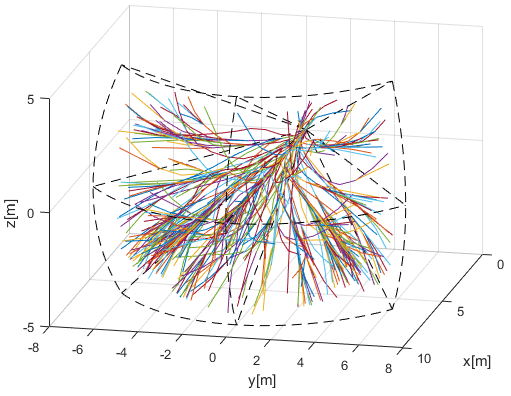
\includegraphics[width=0.7\textwidth]{\FIGDIR/P05ChaoticReachSetMethod}
    \caption{Trajectories for chaotic reach set approximation method}
    \label{fig:P05ChaoticReachSetMethod}
\end{figure}
The \emph{tuning parameter} $c$ is spread ratio, which defines how many nodes should be selected in each cell $c_{i,j,k}$. Example of reduced reach set approximating is given in fig. \ref{fig:P05ChaoticReachSetMethod}. \emph{Overall method performance} for various avoidance grid sizes:
\begin{enumerate}
    \item Don`t keep trajectories smoothness.
    \item Has high coverage. 
    \item Has high count of nodes.
\end{enumerate}

\subsection{Harmonic reach set approximation}\label{s:harmonicApproximationReachSet}
\noindent \emph{Main intention} is to create reduced reach set approximation $\mathscr{R}_R$. The \emph{smoothness} of generated trajectories is main priority. It is known that trajectory going trough cell center has higher probability to be smooth. The cost functional J (\ref{eq:harmonicExpansionCondition}) is product of smoothness function $P_S$ (\ref{eq:smmothnesFunction}) and inverted distance of last trajectory point $\mathscr{T}(\hat{x},B)\to\R^3$ to last passing cell center c.center. 

\begin{equation}\label{eq:harmonicExpansionCondition}
    J(\mathscr{N}(\textbf{x}),B,\mathscr{C}) =  \frac{1}{d(\text{c.center},\mathscr{T}(\hat{x},B)\to\R^3)}\times P_S(\mathscr{T}(\vec{x},B))
\end{equation}

\begin{figure}[H]
    \centering
    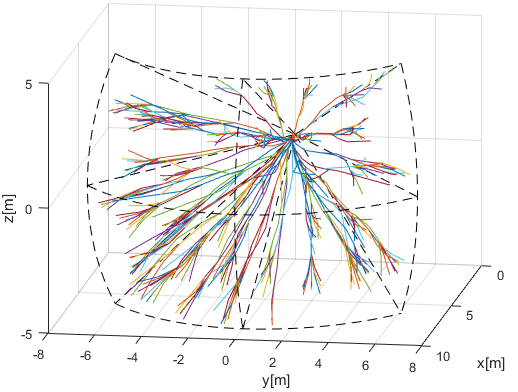
\includegraphics[width=0.7\textwidth]{\FIGDIR/P06HarmonicReachSetMethod}
    \caption{Trajectories for harmonic reach set approximation method}
    \label{fig:P06HarmonicReachSetMethod}
\end{figure}

\noindent \emph{Tuning parameter} $h$ decides how many nodes $\mathscr{N}$ in one cell $c_{i_{l_l},j,k}$ in layer $l_l\subset\mathscr{A}(t_i)$ will be expanded. The example of harmonic reach set is given in fig. \ref{fig:P06HarmonicReachSetMethod}. One can see that almost all trajectories have long straight (smooth) segments. Overall method performance for various avoidance grid sizes:
\begin{enumerate}
    \item Keep trajectories smoothness.
    \item Has low coverage.
    \item Has low count of nodes.
\end{enumerate}

\subsection{Combined reach set approximation}\label{s:combinedReachSetApproximation}
\noindent \emph{Chaotic reach set approximation} (sec. \ref{s:chaoticApproximationReachSet}) lacks smoothness of trajectories for navigation without obstacles, it has great coverage ration $C_R$. \emph{Harmonic reach set approximation} (sec. \ref{s:harmonicApproximationReachSet}) is great for navigation in unconstrained environment, but its coverage capabilities are low.

Because of existence of tuning parameters for \emph{chaotic reach set approximation} $c$ and \emph{harmonic reach set approximation} $h$ \emph{Combined method} can be proposed. Using following approach harmonic tree with expansion tuning parameters $h,c$ can be achieved:
\begin{enumerate}
    \item Create identical root nodes $\mathscr{N}_h(\textbf{x}=\hat{x}(t_i),B=\varnothing,J=0,\mathscr{C}=\varnothing)$ for harmonic expansion and $\mathscr{N}_c(\textbf{x}=\hat{x}(t_i),B=\varnothing,J=0,\mathscr{C}=\varnothing)$ for chaotic expansion.
    \item Expand harmonic root $\mathscr{N}_h$ using maximum criterion $J$ (\ref{eq:harmonicExpansionCondition}) and tuning parameter $h$.
    \item Expand chaotic root $\mathscr{N}_c$ using maximum criterion $J$ (\ref{eq:chaoticExpansionCondition}) and tuning parameter $c$.
    \item Merge chaotic tree with root $\mathscr{N}_c$  and harmonic tree with  root $\mathscr{N}_h$. Merge is possible because both tree structures are compatible and using same structures except expansion criterion (proof omitted). Example of merging multiple trees can be found in \cite{o1996log}.
\end{enumerate}

\begin{figure}[H]
    \centering
    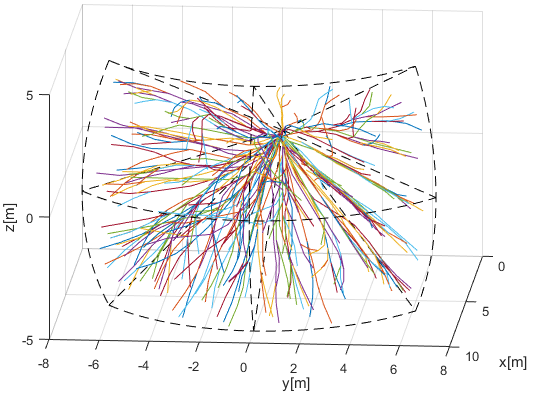
\includegraphics[width=0.7\textwidth]{\FIGDIR/P07CombinedReachSetMethod}
    \caption{Trajectories for combined reach set approximation method}
    \label{fig:P07CombinedReachSetMethod}
\end{figure}

\noindent Example of \emph{harmonic reach set approximation} is protrayed in fig. \ref{fig:P07CombinedReachSetMethod}. Overall method performance for various avoidance grid sizes:
\begin{enumerate}
    \item Keep trajectories smoothness.
    \item Has high coverage.
    \item Has medium count of nodes.
\end{enumerate}







